% \begin{frame}{Open questions}
%     \begin{itemize}
%         \item \(\text{exponent} \leq M_2(n) \leq \text{ double exponent}\)
%         \\Question: Do we need the double exponent at all?
%         \item \(M_d(n)\overset{?}{\leq} \text{ double exponent}\)
%         \item \(\text{polynomial }\leq F_d(n)  \leq \text{double exponent}\)
%         \\Question:  Do we need the double exponent at all?

%     \end{itemize}
    
% \end{frame}
\begin{frame}{Framing it as Ramsey}
    We can frame problems from this paper in the framework of Ramsey numbers.\\
    Take an array \(f:[N]^2\to \mathbb{R}\)  and a hypergraph \(K^3_{N,N}\) of the form \(A \cup B\) with a red, blue colouring edge \(\chi\):
    \begin{columns}
    \begin{column}{0.6\linewidth}
        
    \[\chi(i,j,j')=\begin{cases}
        \text{red if }\space\space  f(i,j)< f(i,j')\\
        \text{blue if }f(i,j)\geq f(i,j') 
    \end{cases}\]
    \end{column}
    \begin{column}{0.3\linewidth}
        \begin{figure}
            \centering
            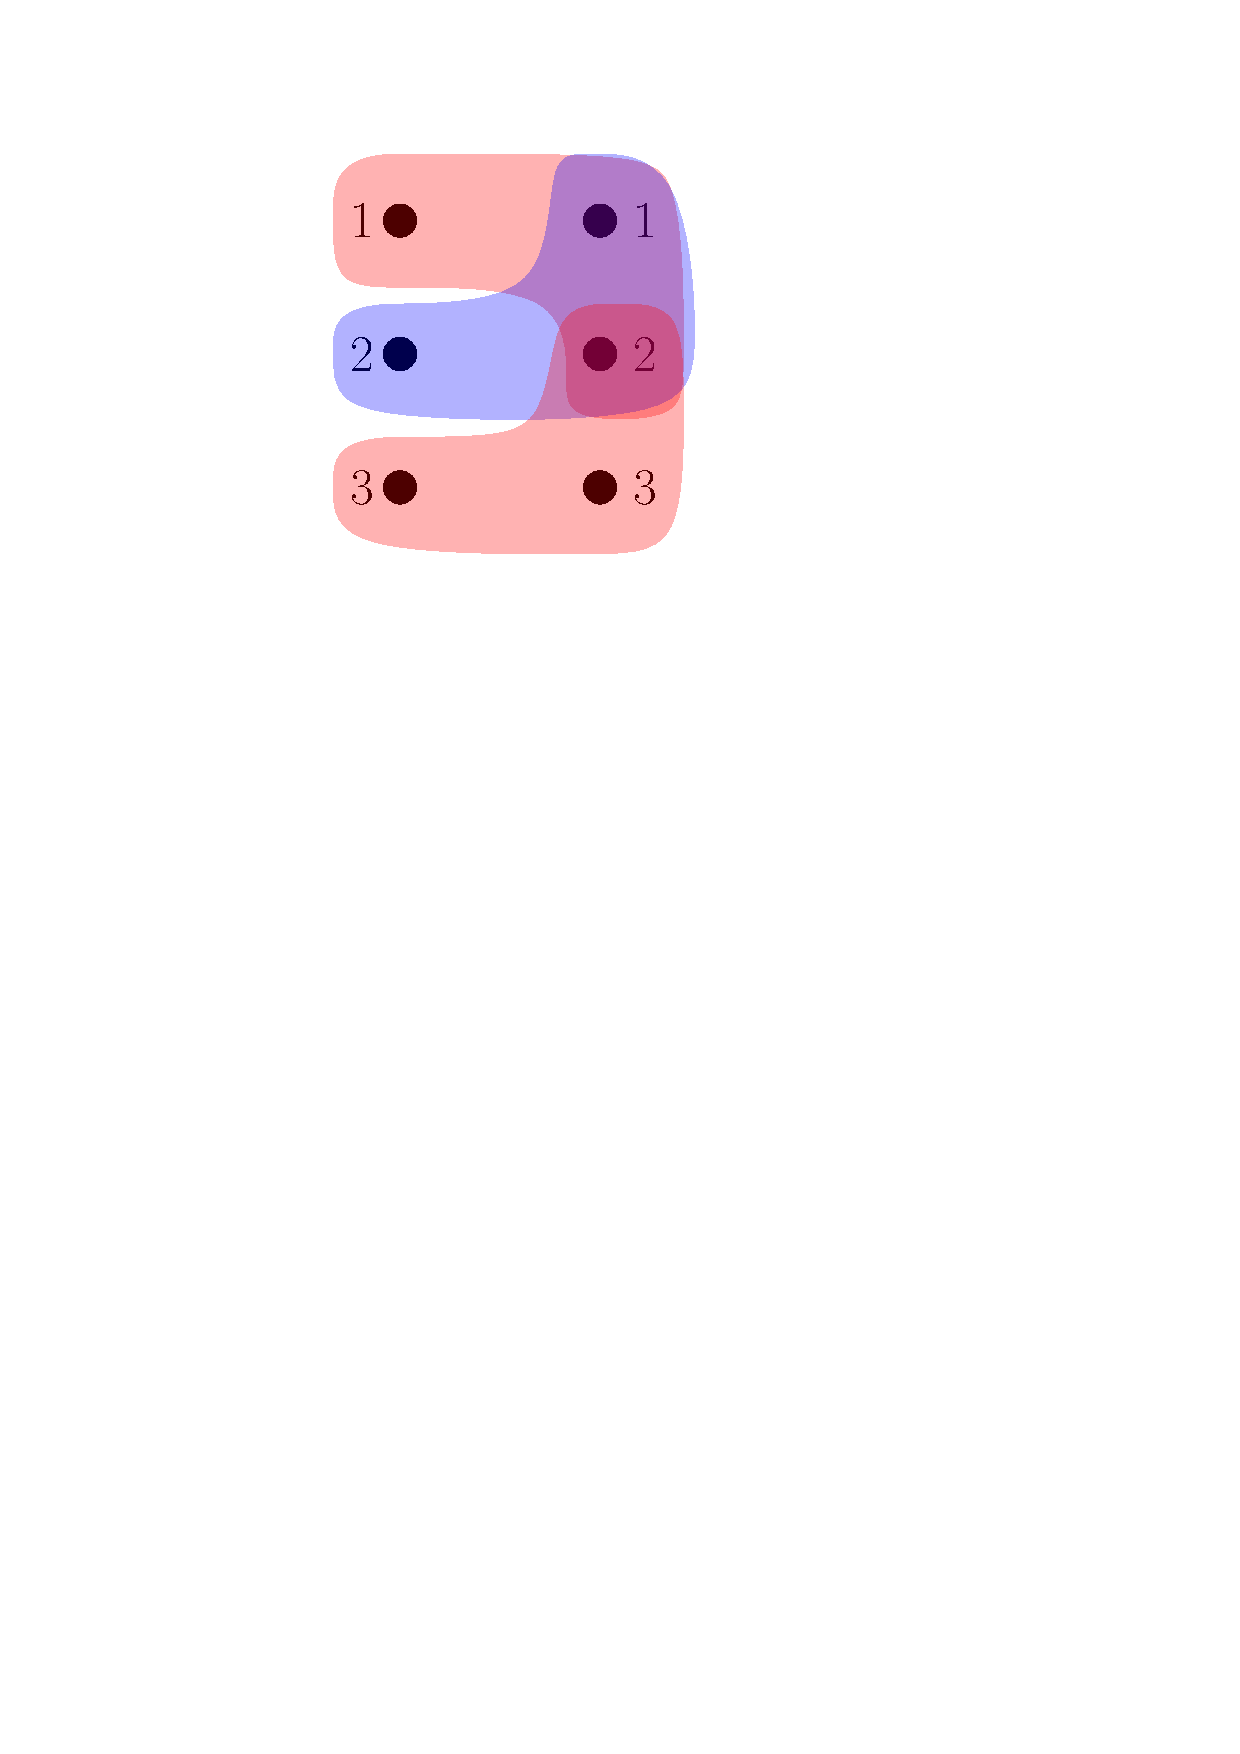
\includegraphics[width=0.5\linewidth]{images/like_ramsey.pdf}
        \end{figure}
    \end{column}
    \end{columns}

    \pause
    Suppose there are two size subsets \(\tilde{a} \subseteq A\) and \(\tilde{b} \subseteq B\) s.t.
    \begin{itemize}
        \item \(\set{a_i, b_j, b_{j+1}}\) is monochromatic under \(\chi\)
        \item \(\set{a_i, a_{i+1}, b_{j}}\) is monochromatic under \(\chi\)
    \end{itemize}
    then \(f\) is a monotone array when restricted to \(\tilde{a}\times \tilde{b}\)
\end{frame}


\begin{frame}{Summary of Bounds}
  \renewcommand{\arraystretch}{1.4}
  \begin{center}
    \begin{tabular}{lccc}
      \toprule
      & \( M_d(n) \) (monotone) & \( F_d(n) \) (mono→lex) & \( L_d(n) \) (lex) \\
      \midrule
      \( d=1 \) & \( (n-1)^2+1 \) & \( 1 \) & \( (n-1)^2+1 \) \\
      \( d=2 \) & \( 2^{2^{(2+o(1))n}} \) & \( 2n^2-5n+4 \) & \( 2^{2^{(4+o(1))n^2}} \) \\
      \( d=3 \) & \( 2^{2^{(2+o(1))n^2}} \) & \( 2^{O(n)} \) & \( 2^{2^{2^{O(n)}}} \) \\
      \( d \geq 4 \) & \( 2^{2^{2^{O_d(n^{d-1})}}} \) & \( 2^{O_d(n^{d-2})} \) & \( \text{towr}_5(O_d(n^{d-2})) \) \\
      \midrule
      lower bd & \multicolumn{3}{c}{\( M_d(n) \geq n^{(1-1/d)n^{d-1}} \)} \\
      \bottomrule
    \end{tabular}
  \end{center}
\end{frame}

\begin{frame}{Open Problems}
  \begin{ffact}{Main open problem}
    What is the order of magnitude of \( M_2(n) \)?
    Is it closer to \emph{exponential} or \emph{double exponential} in \( n \)?
  \end{ffact}
\pause
  \begin{ffact}{Question 4.2}
    For \( d \geq 4 \), is \( M_d(n) \) bounded by a \emph{double exponential}
    in \( n^{d-1} \)?
  \end{ffact}
\pause
  \begin{ffact}{Question 4.3}
    What is the smallest \( N \) such that, given \( N \) increasing \( N \times N \)
    arrays, one can find an \( n \times n \) lex-monotone pattern appearing in the
    same positions in at least \( n \) of the arrays?
    Is \( N \) polynomial or exponential in \( n \)?
  \end{ffact}
\end{frame}
% \begin{frame}{Other generalisations}
%     \begin{theorem}{Theorem (Suk, 2017)}
%         Any \(2^{n+o(n)}\) points in \(\mathbb{R}^2\) contain a convex subset of size \(n\).
%     \end{theorem}
%     \medskip
%     \pause
% \begin{theorem}{Theorem (Xu, 2024)}
% % Any sequence of \(n\) pairwise distinct real numbers contains a \(k\)-
% % modal subsequence of length at least
% % \(\sqrt{(2k + 1)(n − \frac{1}{4} )} - \frac{k}{2}\)
% % \end{theorem}
% % A k-modal sequence is a sequence of real numbers that can be partitioned into k + 1 (possibly
% % empty) monotone sections such that adjacent sections have opposite monotonicities. 
% \end{frame}


